\documentclass[conference]{IEEEtran}
\IEEEoverridecommandlockouts
% The preceding line is only needed to identify funding in the first footnote. If that is unneeded, please comment it out.
\usepackage{cite}
\usepackage{amsmath,amssymb,amsfonts}
\usepackage{algorithmic}
\usepackage{graphicx}
\usepackage{textcomp}
\usepackage{xcolor}
\usepackage{caption}
\usepackage{subcaption}
\def\BibTeX{{\rm B\kern-.05em{\sc i\kern-.025em b}\kern-.08em
    T\kern-.1667em\lower.7ex\hbox{E}\kern-.125emX}}
\begin{document}

\title{Image Processing and Computer Vision\\
}
\author{\IEEEauthorblockN{1\textsuperscript{st} George Lancaster}
\IEEEauthorblockA{\textit{dept. of Computer Science} \\
\textit{University of Bristol}\\
Bristol, United Kingdom \\
qv18258@bristol.ac.uk}
\and
\IEEEauthorblockN{2\textsuperscript{nd} Ren Jiang}
\IEEEauthorblockA{\textit{dept. of Computer Science} \\
\textit{University of Bristol}\\
Bristol, United Kingdom \\
mu18336@bristol.ac.uk}
}


\maketitle

\begin{abstract}
This report outlines the tasks completed for Image Processing and Computer Vision assignment one. The assignment has been split into four sub-tasks. In task one, we experiment with the Viola-Jones object detector to detect faces.
\end{abstract}

\section{The Viola-Jones Object Detector}
We first annotated an image data set containing sixteen images for ground truth. Each image within the data set contains faces, dartboards or a combination of both. In this first task, we use the Viola-Jones object detector to find faces within the images. 
\begin{figure}[htb]
\centering
\begin{subfigure}{.5\linewidth}
  \centering
  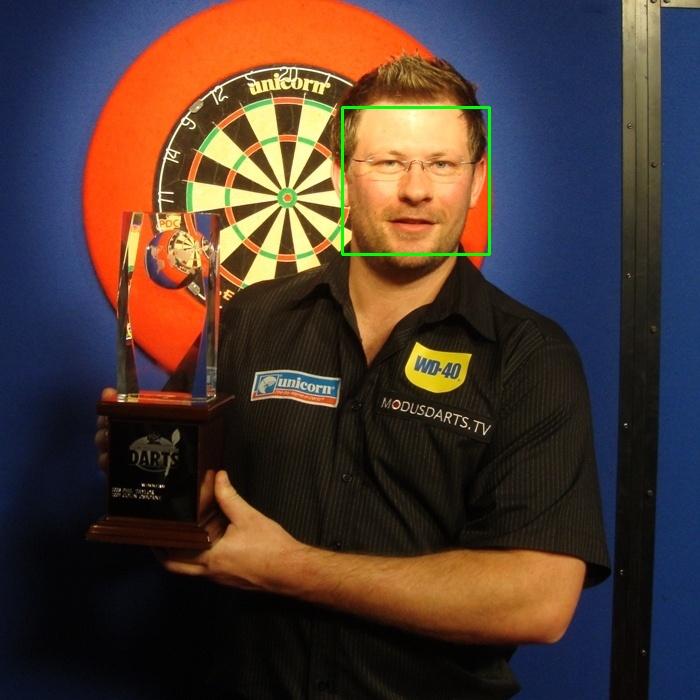
\includegraphics[width=.9\linewidth]{images/detected0.jpg}
  \caption{darts4.jpg}
  \label{fig:sub1}
\end{subfigure}%
\begin{subfigure}{.5\linewidth}
  \centering
  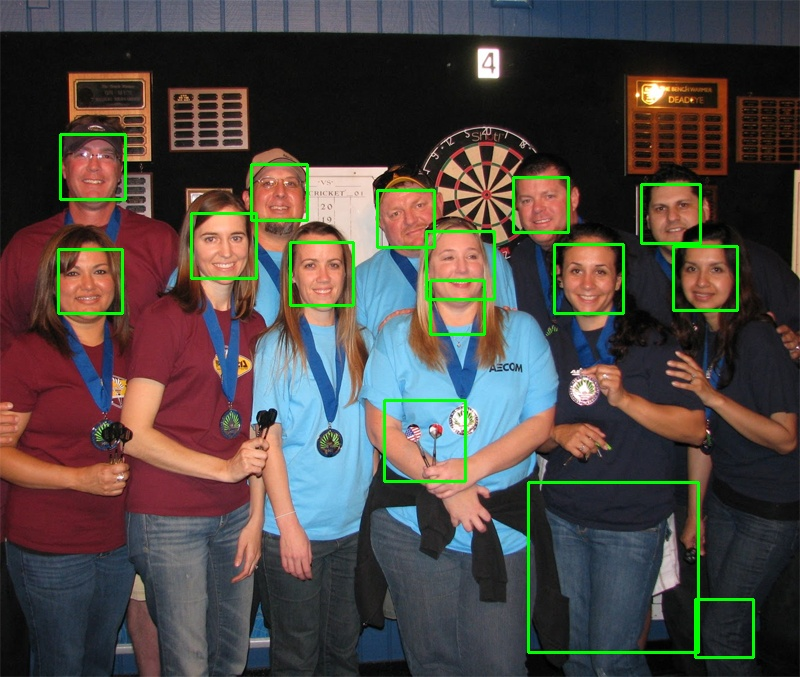
\includegraphics[width=.9\linewidth]{images/detected1.jpg}
  \caption{darts5.jpg}
  \label{fig:sub2}
\end{subfigure}

\begin{subfigure}{.5\linewidth}
  \centering
  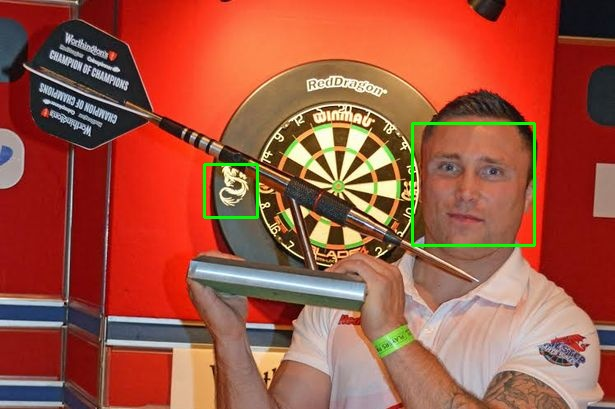
\includegraphics[width=.9\linewidth]{images/detected2.jpg}
  \caption{darts13.jpg}
  \label{fig:sub1}
\end{subfigure}%
\begin{subfigure}{.5\linewidth}
  \centering
  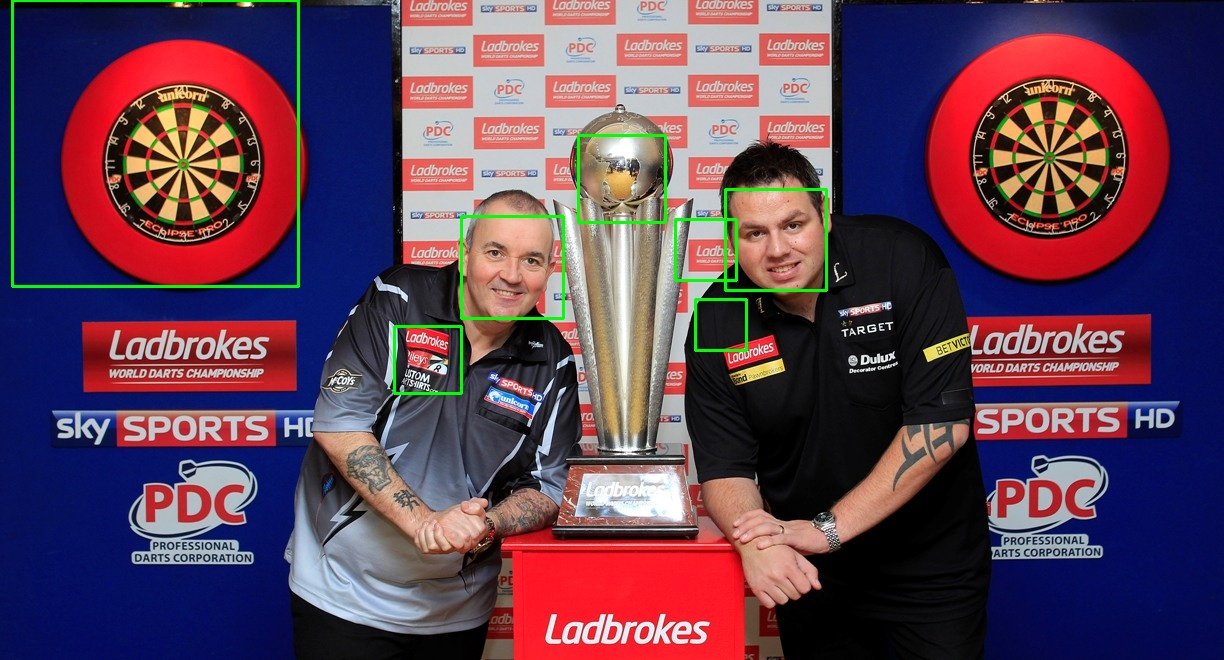
\includegraphics[width=.9\linewidth]{images/detected3.jpg}
  \caption{darts14.jpg}
  \label{fig:sub2}
\end{subfigure}
\begin{subfigure}{.5\linewidth}
\centering
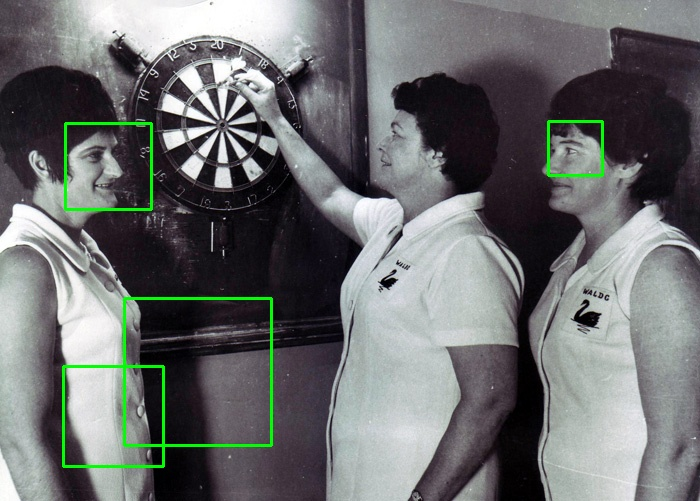
\includegraphics[width=0.9\linewidth]{images/detected4.jpg}
\caption{darts15.jpg}
\end{subfigure}


\caption{Five images from the test data set. Green rectangles have been drawn where the Viola-Jones classifier has detected a face. }
\label{fig:q13}
\end{figure}
\par 
The true positive rate for images \emph{darts5.pg} and \emph{darts15.jpg} are 11 and 1 respectively. 
\par
Practically, the true positive rate is difficult to assess because we because we need to define our own ruleset for what counts as a detection. For this task, we have defined a true detection as an area that shares a 50 per cent overlap with a ground truth label. This value was chosen to maximise the f1 score when classifying faces from the test data set. The results varying the percentage overlap can be seen in table x. 
\par 
\begin{table}[!htp]
\caption{All values of percentage overlap gave an identical F1 score, when detecting faces from the test data set. }
\begin{center}
\begin{tabular}{||c|c||}
\hline
Overlap Threshold (\%) 	& F1 score 	\\ \hline
0 					& 0.568		\\
60 					& 0.541		\\
65					& 0.541		\\
68					& 0.541		\\
69					& 0.519		\\
70 					& 0.514		\\
80					& 0.459		\\ \hline
\end{tabular}
\end{center}
\label{default}
\end{table}%

\par
Although the true positive rate can be used to indicate a classifiers accuracy, it does not reflect its true performance. It is always possible to get a 100 per cent detection rate on any classification task as we can select all possible areas of an image, regardless if they contain a target or not. The key to a good classifier is to get a high true positive rate, whilst keeping the false positives minimal. We can use the F1 score to measure the relationship between the precision and the recall of the model. The F1 score can therefore be considered to be a more reliable measure of classifier performance.
\par
The F1 score of the Viola-Jones classifier, when detecting faces in the test data set is 


\newpage
\section{The Dartboard Detector}
\subsection{Subtask a}
\begin{figure}[htbp]
\begin{center}
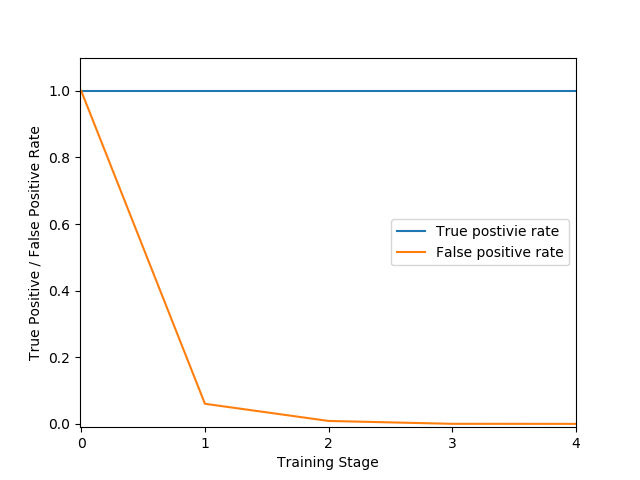
\includegraphics[width=\linewidth]{images/TPRvsFPR}
\caption{True positive rate plotted against false positive rate, when training the cascade classifier on images of dartboards. Each stage of training has been plotted as its own point.}
\label{default}
\end{center}
\end{figure}

\begin{table}[htp]
\caption{F1 scores for all images, when detecting for dartboards using a cascade classier trained on dartboards.}
\begin{center}
\begin{tabular}{||c|c||}
\hline
Image Name 		& F1 Score 	\\ \hline
dart0.jpg			& 0.5	00		\\
dart1.jpg			& nan		\\
dart2.jpg			& 0.250		\\
dart3.jpg			& 1.538		\\
dart4.jpg			& 0.4	00		\\
dart5.jpg			& 0.154		\\
dart6.jpg			& 0.333		\\
dart7.jpg			& nan		\\
dart8.jpg			& 0.160		\\
dart9.jpg			& 0.222		\\
dart10.jpg			& 0.400		\\
dart11.jpg			& 0.222		\\
dart12.jpg			& 0.667		\\
dart13.jpg			& 0.200		\\
dart14.jpg			& 0.087		\\
dart15.jpg			& 0.667		\\ \hline
Average f1 score 	& 0.276		\\ \hline
\end{tabular}
\end{center}
\label{default}
\end{table}%
\newpage
\section{Integration with Shape Detectors}
\newpage
\section{Further Improvements}






\end{document}